%-----------------------------------------------------------------------------%
\chapter{\babEmpat}
%-----------------------------------------------------------------------------%

Pada bab ini akan dibahas tentang hasil penelitian dari metodologi yang ada pada bab tiga, dan masalah-masalah yang dihadapi pada saat implementasinya dan pembahasannya.


%-----------------------------------------------------------------------------%
\section{Overview Metodologi}
%-----------------------------------------------------------------------------%
Model yang dihasilkan dari \textit{unsupervised learning} yang dilakukan oleh DBN menggunakan data training, harus diuji dahulu dengan dengan data validasi dan data testing, yaitu dengan cara memberikan satu layer output menggunakan \textit{logistic regression} hal ini untuk mengetahui apakah klasifikasinya lebih baik atau sebaliknya. Hasil ini berpengaruh pada proses tuning parameter (jumlah layer dan jumlah hidden unitnya) untuk didapatkan \textit{cost} yang paling optimal pada saat pre-training. Setelah dilakukan perankingan secara multi-step dari hasil percobaan yang terbaik, diperlukan pengujian apakah apakah seleksi fitur tersebut mendapatkan hasil klasifikasi yang lebih baik dengan menggunakan fitur yang telah diseleksi saja. Dengan cara membandingkan \textit{biomarker} yang ditemukan oleh algoritma multi-step rangking dibandingkan dengan algoritma yang ada di literatur yaitu metode bonferroni untuk melakukan test statistik pada data gen tersebut \citep{hochberg1988sharper}. 


%-----------------------------------------------------------------------------%
\section{Hasil Percobaan DBN Dengan Setting Hyperparameter yang Berbeda}
%-----------------------------------------------------------------------------%
Untuk mendapatkan hasil yang optimal dibutuhkan banyak percobaan dan setting parameter yang berbeda-beda, mulai dari jumlah layer, jumlah hidden unit tiap layernya, learning rate, banyaknya gibbs step dan ukuran batch-nya. Oleh karena itu, dibawah adalah rekapitulasi percobaan dengan hasil terbaik dari sekian percobaan, dipilih lima percobaan yang paling baik hasilnya untuk emudian dianalisa lebih jauh. Percobaan dibawah memiliki setting parameter seperti pada daftar berikut:


% Please add the following required packages to your document preamble:
% \usepackage{booktabs}
\begin{table}
\centering
\caption{Setting Parameter Awal}
\label{tab:var}
\begin{tabular}{@{}lll@{}}
\toprule
No. & Item          & Keterangan                                                                                                                                                \\ \midrule
1   & Dataset       & \begin{tabular}[c]{@{}l@{}}Gene expression signature of cigarette smoking \\ and its role in lung adenocarcinoma development \\ and survival \citep{landi2008gene} \end{tabular} \\
2   & Total Data    & 107 Pasien                                                                                                                                                \\
3   & Kanker        & 58 Pasien                                                                                                                                                 \\
4   & Normal        & 49 Pasien                                                                                                                                                 \\
5   & Training      & 69 Pasien                                                                                                                                                 \\
6   & Validasi      & 14 Pasien                                                                                                                                                 \\
7   & Testing       & 20 Pasien                                                                                                                                                 \\
8   & Epoch         & 1000 dan 2000                                                                                                                                             \\
9   & Learning Rate & 0.01                                                                                                                                                      \\
10  & Fitur Gen     & 22.283 Gen                                                                                                                                                \\ \bottomrule
\end{tabular}
\end{table}
Setelah dilakukan eksperimen secara \textit{unsupervised} diperoleh \textit{cost} terbaik pada Percobaan dan hasilnya ada di tabel \ref{tab:dbn} :


\begin{table}
\centering
\caption{Eksperimen DBN Unsupervised}
\label{tab:dbn}
\tabcolsep=0.11cm
\begin{tabular}{@{}llllllll@{}}
\toprule
\multicolumn{1}{c}{Eks} & \multicolumn{1}{c}{Hidden} & \multicolumn{1}{c}{Epoch} & \multicolumn{1}{c}{Cost Lyr 0} & \multicolumn{1}{c}{Cost Lyr 1} & Cost Lyr 2 & Cost Lyr 3 & Waktu (Jam) \\ \midrule
1 & \begin{tabular}[c]{@{}l@{}}{[}10000, 5000,\\  1000, 500{]}\end{tabular} & 1000 & -12888.2 & -1.37401 & -3499.73 & -0.351105 & 65 \\
 &  & 2000 & -12888.2 & -0.828167 & -3484.73 & -0.150991 & 132 \\
2 & \begin{tabular}[c]{@{}l@{}}{[}7000, 10000, \\ 5000, 1000{]}\end{tabular} & 1000 & -12886.8 & -1.36201 & -6866.37 & -0.163702 & 63 \\
 &  & 2000 & -12886.7 & -1.57877 & -6873.31 & -0.0729352 & 138 \\
3 & \begin{tabular}[c]{@{}l@{}}{[}3000, 2000, \\ 1000, 100{]}\end{tabular} & 1000 & -12897.8 & -0.862442 & -1410.18 & -3.244 & 58 \\
 &  & 2000 & -12897.0 & -0.849616 & -1397.09 & -3.14657 & 123 \\
4 & \begin{tabular}[c]{@{}l@{}}{[}15000, 8000, \\ 2000{]}\end{tabular} & 1000 & -12934.5 & -32.4227 & -2756.41 & - & 68 \\
5 & \begin{tabular}[c]{@{}l@{}}{[}25000, 17000, \\ 7000{]}\end{tabular} & 1000 & -12888.1 & -12.1715 & -5446.34 & - & 72 \\ \bottomrule
\end{tabular}
\end{table}



Tabel diatas menunjukkan bahwa dengan epoch 1000 dan 2000 costnya tidak menunjukkan perbaikan secara signifikan. Bahkan untuk beberapa kasus, hasilnya lebih buruk. Dibawah adalah plot cost untuk percobaan yang dilakukan secara \textit{greedy layer wise}, dari plot tersebut dapat dilihat bahwa cost pada epoch 700-an sudah tidak lagi membaik secara signifikan. Hal ini bisa dikarenakan oleh terbatasnya data training yang dipakai yaitu hanya 69 pasien dikarenakan oleh terbatasnya data yang didapatkan karena mahalnya percobaan microarray itu sendiri.

\subsection{Plot Cost Percobaan 1}

\begin{figure}
	\centering
	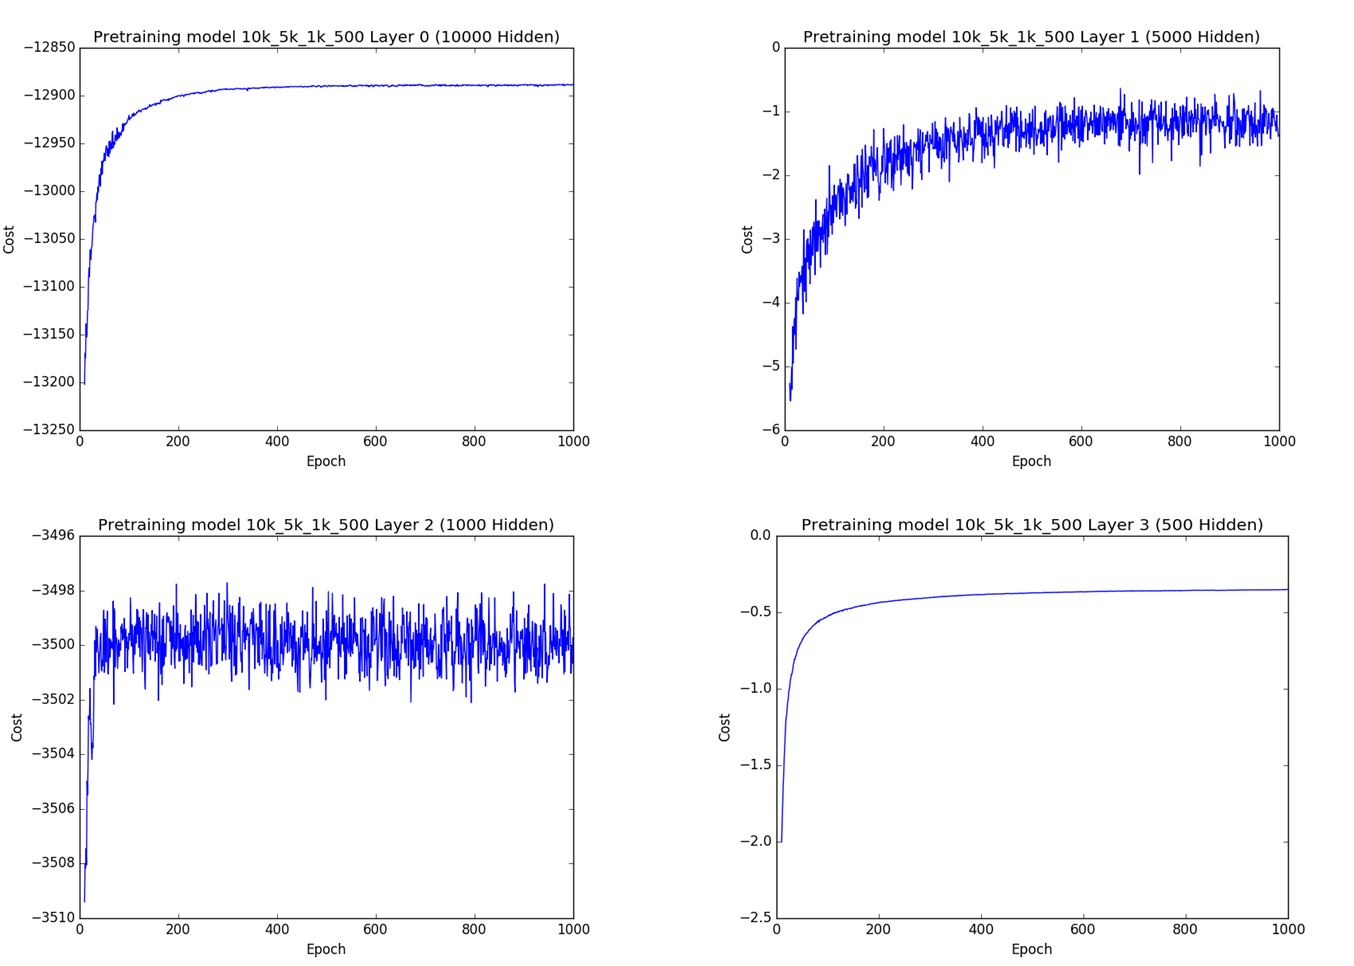
\includegraphics[width=0.9\textwidth]
		{pics/percobaan_1.png}
	\caption{Perbandingan Cost Pada Percobaan 1 Sampai 1000 Epoch Pada Tiap Layernya}
	\label{fig:percobaan1}
\end{figure}

Pada \pic~\ref{fig:percobaan1} merupakan perbandingan cost dari layer 0 sampai 3 (4 layer) dengan konfigurasi hidden [10000, 5000,1000,500] disitu bisa dilihat bahwa setelah epoch 500 tidak terjadi perbaikan cost yang signifikan. Juga cost pada layer 2 dan 3 memiliki ritme yang tidak stabil.

\subsection{Plot Cost Percobaan 2}
\begin{figure}
	\centering
	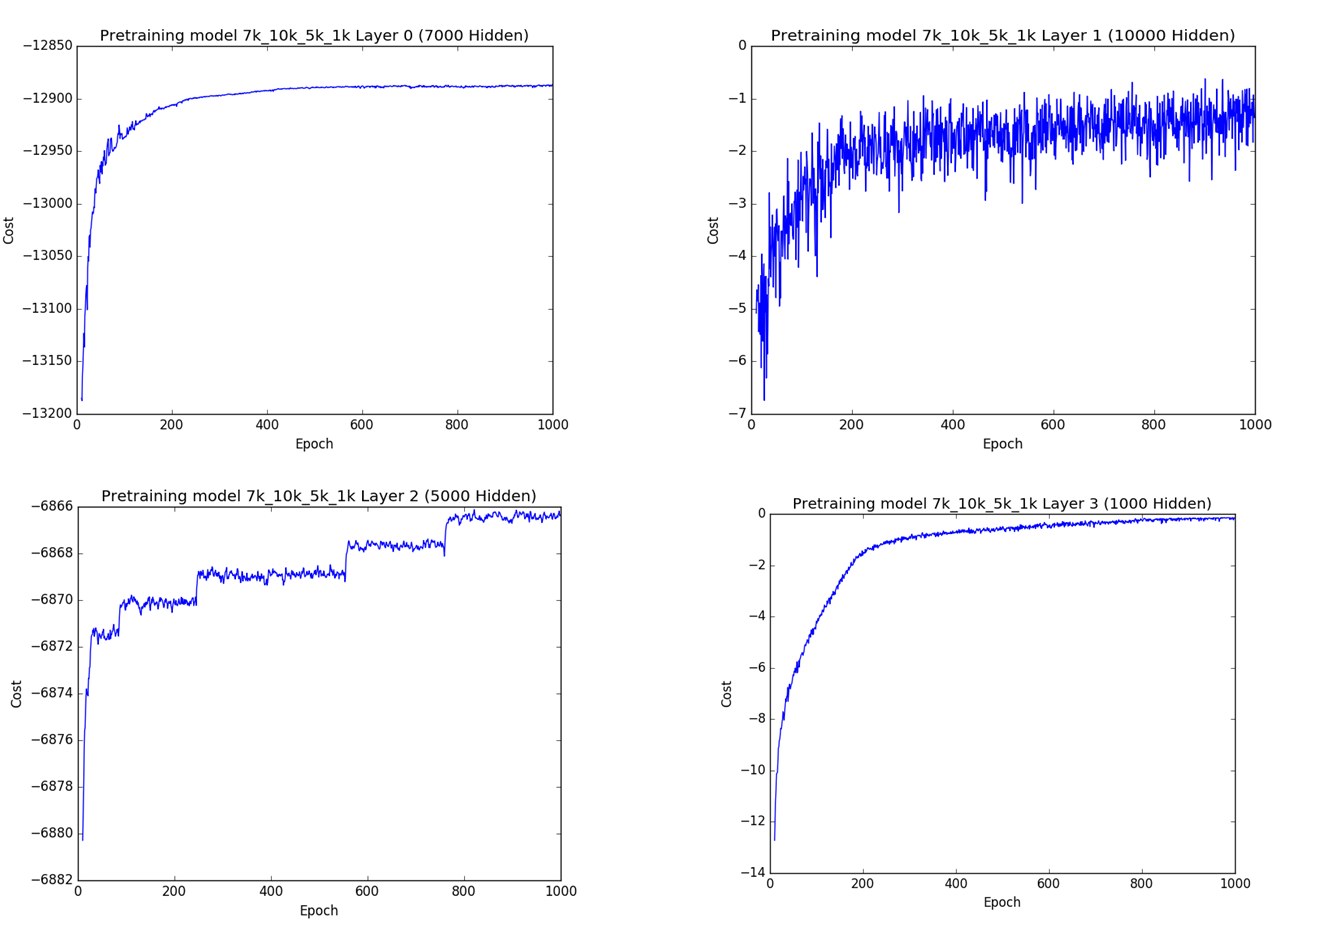
\includegraphics[width=0.9\textwidth]
		{pics/percobaan_2.png}
	\caption{Perbandingan Cost Pada Percobaan 2 Sampai 1000 Epoch Pada Tiap Layernya}
	\label{fig:percobaan2}
\end{figure}

Pada \pic~\ref{fig:percobaan2} merupakan perbandingan cost dari layer 0 sampai 3 (4 layer) disitu bisa dilihat bahwa setelah epoch 500 tidak terjadi perbaikan cost yang signifikan. Juga cost pada layer 2 dan 3 memiliki ritme yang juga tidak stabil.

\subsection{Plot Cost Percobaan 3}
\begin{figure}
	\centering
	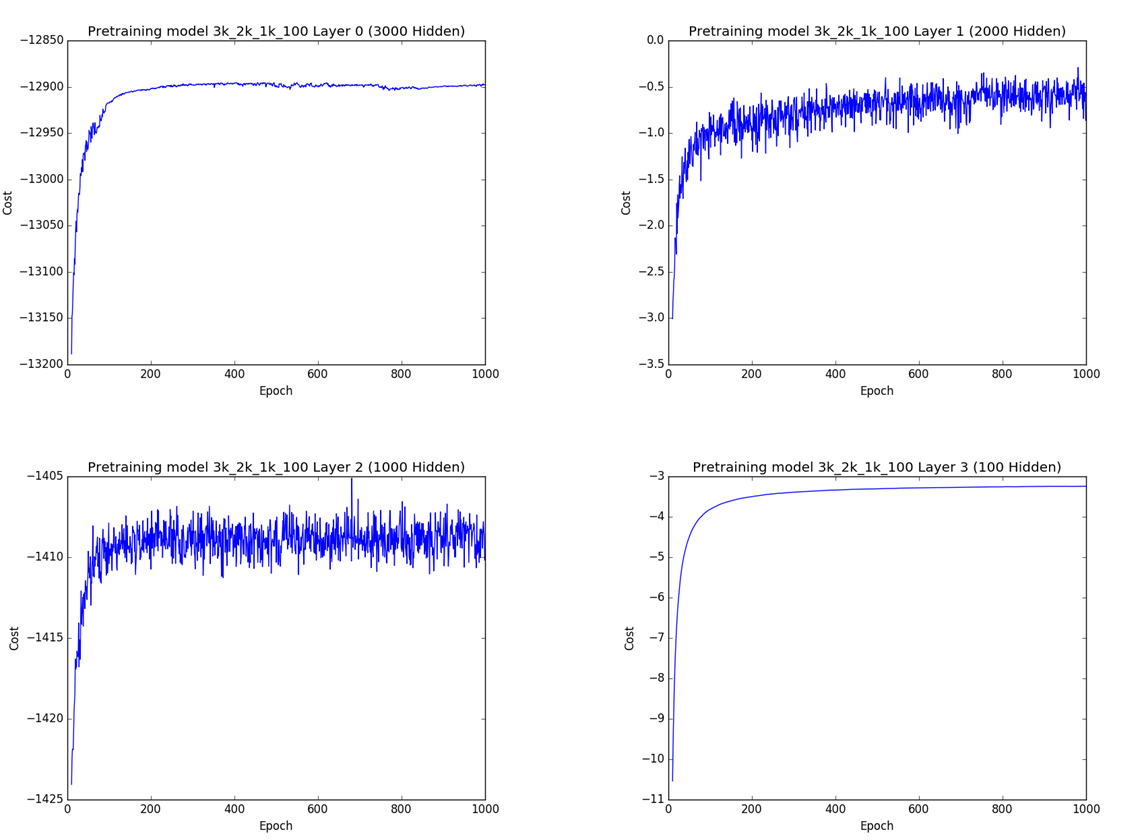
\includegraphics[width=0.9\textwidth]
		{pics/percobaan_3.png}
	\caption{Perbandingan Cost Pada Percobaan 3 Sampai 1000 Epoch Pada Tiap Layernya}
	\label{fig:percobaan3}
\end{figure}
Pada \pic~\ref{fig:percobaan3} merupakan perbandingan cost dari layer 0 sampai 3 (4 layer) disitu bisa dilihat bahwa setelah epoch 500 tidak terjadi perbaikan cost yang signifikan. Juga cost pada layer 2 dan 3 memiliki ritme yang tidak stabil.

Berarti dari ketiga percobaan tersebut, secara garis besar, epoch lebih dari 700-an tidak mempengaruhi perbaikan error rekonstruksinya. Hal ini bisa disebabkan karena kurangnya data training.


%-----------------------------------------------------------------------------%
\section{Hasil Penerapan Multi Step Ranking Bobot}
%-----------------------------------------------------------------------------%

Percobaan training DBN secara \textit{unsupervised} yang dilakukan dengan setting pada tabel \ref{tab:dbn} diatas dipilih tiga percobaan terbaik untuk dilakukan algoritma multi-step ranking.

\subsection{Diagram Venn Perpotongan Percobaan 1, 2 dan 3}

Pada saat dilakukan multi-step ranking pada percobaan 1, 2 dan 3. Dibuat perankingan top 250 gen yang paling berpengaruh terhadap model-nya masing-masing. Kemudian, dibuat sebuah diagram untuk mendapatkan perpotongan 250 gen tersebut pada tiap-tiap percobaan. Hal ini digunakan untuk mengetahui gen-gen mana yang selalu muncul di percobaan 1,2,3 atau muncul di dua percobaan dan hanya muncul di satu percobaan. Maka didapatkan diagram venn seperti pada \pic~\ref{fig:venn1}

\begin{figure}
	\centering
	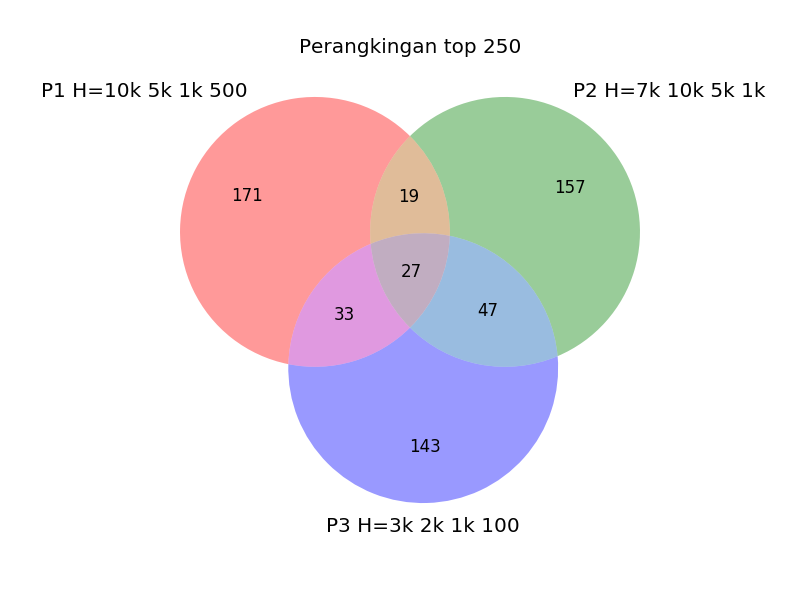
\includegraphics[width=0.9\textwidth]
		{pics/venn1.png}
	\caption{Perbandingan Perankingan Top 250 pada tiga percobaan yang paling baik, ada 27 gen yang selalu muncul pada ketiga percobaan tersebut}
	\label{fig:venn1}
\end{figure}
Pada diagram venn diatas, ditunjukkan bahwa ada 27 gen yang selalu muncul pada percobaan 1, 2, 3. Hal ini menunjukkan bahwa gen tersebut adalah gen yang diindikasikan lebih informatif dibandingkan dengan gen yang lainnya. Ke 27 gen tersebut ada pada tabel \ref{tab:indexgen} penemuan 27 gen yang selalu muncul pada tiga percobaan terbaik tersebut bisa diindikasikan sebagai \textit{biomarker}. Yaitu gen yang bisa mencirikan seseorang terkena kanker paru-paru atau tidak.\\


% Please add the following required packages to your document preamble:
% \usepackage{booktabs}
\begin{table}
\centering
\caption{Index dan Kode Gen yang Diindikasikan sebagai \textit{Biomarker}}
\label{tab:indexgen}
\begin{tabular}{@{}ll@{}}
\toprule
Index & Kode Gen      \\ \midrule
7303  & 207783\_x\_at \\
1418  & 201891\_s\_at \\
9666  & 210183\_x\_at \\
15890 & 216520\_s\_at \\
24    & 200004\_at    \\
21919 & 38691\_s\_at  \\
11298 & 211911\_x\_at \\
13741 & 214363\_s\_at \\
46    & 200026\_at    \\
307   & 200780\_x\_at \\
12727 & 213347\_x\_at \\
13246 & 213867\_x\_at \\
4418  & 204892\_x\_at \\
6084  & 206559\_x\_at \\
13765 & 214387\_x\_at \\
328   & 200801\_x\_at \\
201   & 200674\_s\_at \\
21860 & 37004\_at     \\
101   & 200081\_s\_at \\
232   & 200705\_s\_at \\
11370 & 211984\_at    \\
879   & 201352\_at    \\
11120 & 211720\_x\_at \\
20968 & 221607\_x\_at \\
115   & 200095\_x\_at \\
1019  & 201492\_s\_at \\
511   & 200984\_s\_at \\ \bottomrule
\end{tabular}
\end{table}

Ke-27 gen pada tabel tersebut merupakan gen yang diindikasikan memiliki pengaruh yang signifikan pada percobaan. Akan tetapi hal ini perlu dilakukan konfirmasi lebih lanjut untuk memastikan bahwa gen tersebut memang berpengaruh secara signifikan terhadap penyakit kanker paru-paru. Ada dua tahapan konfirmasi yang pertama tahap konfirmasi dengan memastikan bahwa hasil klasifikasi dengan hanya menggunakan top 250 gen tersebut bisa mengklasifikasikan pasien sehat dan pasien kanker. Tahap yang kedua adalah dengan cara konfirmasi melalui literatur tentang biomarker kanker paru-paru yang sudah ditemukan pada penelitian sebelumnya.

%-----------------------------------------------------------------------------%
\section{Bagian Supervised Learning Dengan Multi Layers Perceptron (MLP)}
%-----------------------------------------------------------------------------%



Setelah dilakukan perbandingan gen biomarker yang ditemukan pada proses perankingan diatas, top 250 gen tersebut dibuat menjadi data input untuk kasus klasifikasi. Untuk di evaluasi apakah hasil klasifikasinya lebih baik dibandingkan dengan tanpa seleksi fitur.\\
Tabel \ref{tab:tabel4.2} merupakan perbandingan error antara logistic regression yang ditempatkan pada layer akhir DBN, tanpa dilakukan seleksi fitur. Dibandingkan dengan MLP yang memiliki 1 layer hidden dan 250 hidden unit. Untuk dilakukan training ulang dan dibandingkan dengan hasil yang diperoleh dari logistic regression.

\begin{table}
\centering
\caption{Perbandingan Error Antara Dengan dan Tanpa Seleksi Fitur}
\label{tab:tabel4.2}
\begin{tabular}{@{}lllll@{}}
\toprule
 & \multicolumn{2}{l}{Tanpa Seleksi Fitur(LogReg)} & \multicolumn{2}{l}{Dengan Seleksi Fitur(MLP)} \\ \midrule
Percobaan & Validation Error & Test Error & Validation Error & Test Error \\
1 & 50\% & 66\% & 5.55\% & 0\% \\
2 & 50\% & 30\% & 0\% & 8.33\% \\
3 & 50\% & 30\% & 0\% & 16\% \\ \bottomrule
\end{tabular}
\end{table}

Dari tabel \ref{tab:tabel4.2} dapat disimpulkan bahwa terjadi perbaikan signifikan antara validation dan test error dibandingkan tanpa dilakukan seleksi fitur. Akan tetapi hal ini masih belum menunjukkan apakah seleksi fitur gen tersebut merupakan \textit{biomarker}. Oleh karena itu diperlukan evaluasi lebih lanjut yaitu dengan evaluasi literatur untuk memastikan bahwa gen yang ditemukan memang informatif untuk kasus kanker paru-paru.

%-----------------------------------------------------------------------------%
\section{Hasil Evaluasi Dengan Literatur Pertama Bonferroni Method\citep{hochberg1988sharper}}
%-----------------------------------------------------------------------------%

Metode Bonferroni adalah metode multipel testing di statistik yang paling umum digunakan untuk dataset dari percobaan \textit{microarray}. Metode ini adalah metode yang dipakai oleh \cite{landi2008gene} dalam menganalisa dataset GSE10072 yang merupakan hasil eksperimen kanker paru-paru \citep{landi2008gene} Dengan melakukan test statistik menggunakan metode bonferroni dipilih 250 gen yang paling signifikan dari hasil test statistik tersebut dibandingkan dengan gen yang dipilih dari metode multi-step ranking, didapatkan hasil sebagai berikut.

\begin{figure}
	\centering
	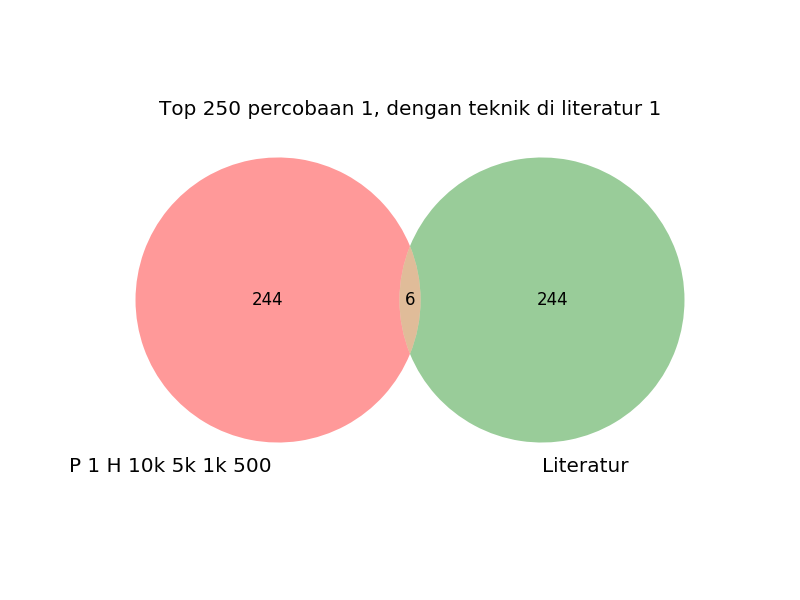
\includegraphics[width=0.9\textwidth]
		{pics/bon1.png}
	\caption{Hasil top 250 Gen dibandingkan dengan Metode bonferroni}
	\label{fig:bon1}
\end{figure}

Pada percobaan 1, dihasilkan perpotongan 6 gen. Walaupun kelihatan kecil tetapi perpotongan 6 gen dari 22 ribu-an gen menjadi sangat signifikan untuk diteliti lebih lanjut gen-gen tersebut sebagai kandidat \textit{Biomarker}

\begin{figure}
	\centering
	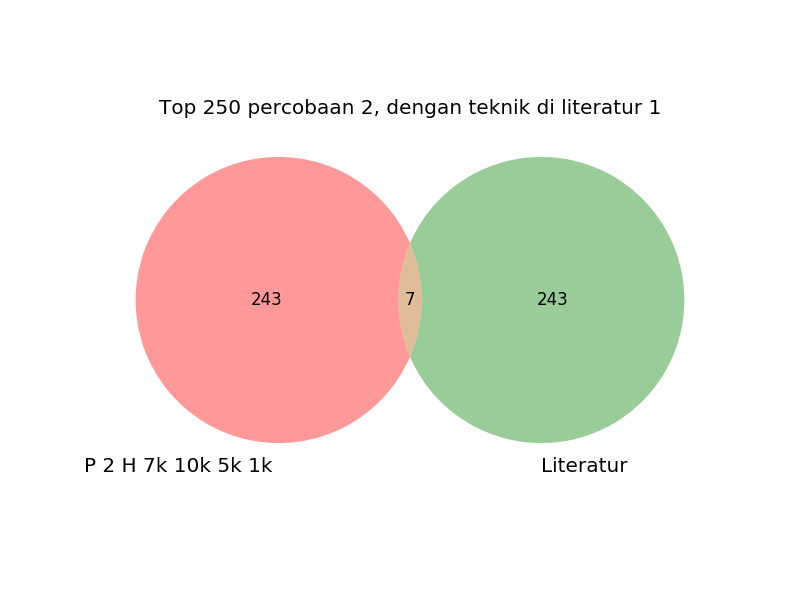
\includegraphics[width=0.9\textwidth]
		{pics/bon2.png}
	\caption{Hasil top 250 Gen dibandingkan dengan Metode bonferroni}
	\label{fig:bon1}
\end{figure}

Percobaan 2 dibandingkan dengan metode bonferroni juga memiliki perpotongan yang tidak besar yaitu 7 gen saja.

\begin{figure}
	\centering
	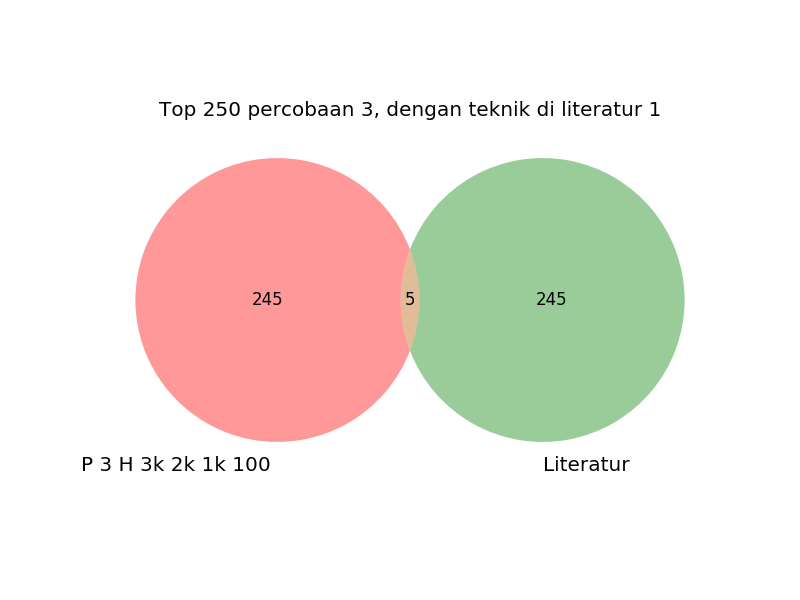
\includegraphics[width=0.9\textwidth]
		{pics/bon3.png}
	\caption{Hasil top 250 Gen dibandingkan dengan Metode bonferroni}
	\label{fig:bon3}
\end{figure}

Percobaan 3 dibandingkan dengan metode bonferroni memiliki perpotongan kesesuaaina 5 gen.



%-----------------------------------------------------------------------------%
\section{Hasil Konfirmasi Dengan Literatur Kedua Harvard Cancer Center (https://ccib.mgh.harvard.edu/xavier)}
%-----------------------------------------------------------------------------%
Sebanyak 27 gen yang ditemukan untuk irisan tiga percobaan terbaik, akan dilakuan review literatur lebih jauh. Menurut situs harvard cancer center, gen-gen tertentu bisa menununjukkan tingkat signifikansi gen tersebut terhadap sebuah penyakit kanker. Sebagai contoh gen yang berada pada ranking 1 pada 27 gen tersebut memiliki signifikasni yang tinggi terhadap kanker paru-paru dibandingkan dengan gen yang dipilih secara acak.
\begin{figure}
	\centering
	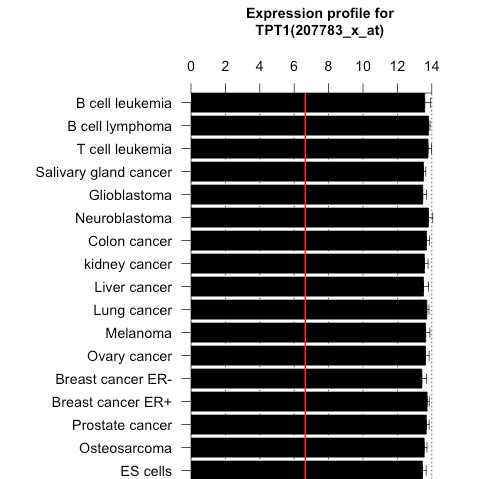
\includegraphics[width=0.9\textwidth]
		{pics/tpt1.png}
	\caption{Profil Ekspresi Gen TPT1 yang merupakan ranking pertama}
	\label{fig:tpt1}
\end{figure}
Dari gambar bisa dilihat bahwa signifikansi gen TPT1 yang merupakan gen dengan ranking pertama memiliki signifikansi terhadap penyakit kanker paru-paru (lung cancer). Sumber profil gen didapat dari 

\begin{figure}
	\centering
	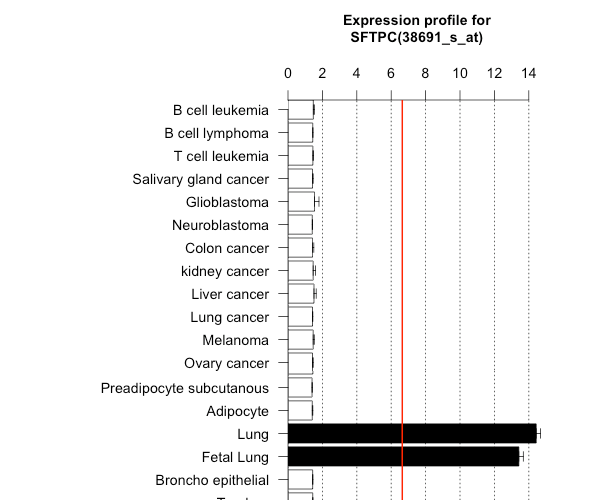
\includegraphics[width=0.9\textwidth]
		{pics/38691_s_at_profil.png}
	\caption{Profil Ekspresi Gen TPT1 yang merupakan ranking pertama}
	\label{fig:SFTPC}
\end{figure}

Pada dua contoh profil yang ditemukan yaitu gen TPT1 dan gen SFTPC bisa disimpulkan bahwa walaupun ekspresi gen tersebut ditemukan pada kanker paru-paru, tetapi tidak unik dan juga ditemukan di kanker-kanker yang lain misalnya leukemia, lymphoma dan sebagainya. Hal ini terjadi karena data yang dipakai adalah data kanker paru-paru saja. Sehingga menemukan biomarker yang unik pada kanker paru-paru saja.
%-----------------------------------------------------------------------------%
\section{Kendala-Kendala yang Dialami Selama Melakukan Percobaan}
%-----------------------------------------------------------------------------%
Pada saat melakukan percobaan dengan menggunakan arsitektur \textit{deep learning} kendala yang paling utama adalah lamanya waktu training dan penggunaan resource memory yang sangat besar. Dengan menggunakan komputer core i5 dengan memory vga 2 GB, dan RAM 4 GB diperlukan waktu rata-rata 3-5 hari. Seperti pada tabel \ref{tab:runtime}. Dikarenakan oleh kendala ini maka untuk melakukan percobaan dengan arsitektur yang lebih besar, misalnya dilakukan penambahan layer (lebih dari 4 layer) dan penambahan hidden unit, menjadi terbatas. Juga masalah pada terbatasnya dataset untuk training yang hanya 107 sampel pasien, hal ini disebabkan oleh mahalnya percobaan \textit{microarray} yang dilakukan sehingga sulit untuk mendapatkan data yang lebih besar lagi.

\begin{table}
\centering
\caption{tabel ukuran model dan waktu running}
\label{tab:runtime}
\begin{tabular}{@{}llll@{}}
\toprule
Percobaan & \begin{tabular}[c]{@{}l@{}}Konfigurasi Hidden\\ (h0, h1, h2, h3)\end{tabular} & Ukuran Model  & \begin{tabular}[c]{@{}l@{}}Running (Jam)\\ (1000e, 2000e)\end{tabular} \\ \midrule
1         & 10000, 5000,1000, 500                                                         & 1 GB          & 65, 132                                                                \\
2         & 7000,10000,5000,1000                                                          & 1 GB          & 63, 138                                                                \\
3         & 3000,2000,1000,100                                                            & 275 MB        & 58, 123                                                                \\
4         & 15000,8000,2000                                                               & Out of Memory & -                                                                      \\
5         & 25000, 17000, 7000                                                            & Out of Memory & -                                                                      \\ \bottomrule
\end{tabular}
\end{table}

Pada tabel diatas, bisa dihilhat bahwa hidden yang melebihi 15000 sudah menghabiskan RAM komputer yang hanya berukuran 4 GB. Oleh karena itu, percobaan yang seharusnya bisa memperdalam layer dan memperbesar hidden unit tidak memungkinkan untuk dilakukan.





